% !TeX root = ..\essay.tex

\section{Evaluation}
\label{ch:evaluation}

\subsection{Evaluation setting}
To evaluate the summaries they were manually annotated.
Each summary has been annotated by at least two raters with the following criteria:

\begin{table}[H]
	\begin{tabularx}{\textwidth}{l|X} \toprule
		criteria            & description \\ \midrule
		Grammaticality      & The sentences should be grammatically correct and not contain obviously ungrammatical sentences that make the text difficult to read.\\
		Non-Redundancy      & There should be no unnecessary repetition in the summary.\\
		Referential Clarity & It should be easy to identify who or what the pronouns and noun
  phrases in the summary are referring to.\\
		Focus               & Sentences should only contain information that is related to the rest of the summary.\\
		Structure           & The summary should be well structured.\\
		Coherence           & The summary should be build from sentence to sentence into a coherent body of information about the topic.\\
		Readability         & The sentences should be readable. This includes the number of words per sentence, average grade level of words and characters per word. \\
		Information Content & The summary should contain enough information about the topic.\\
		Spelling            & The sentences should have no datelines, system-internal formatting, capitalization errors or misspelled words.\\
		Length              & The length of the summary should be within the limit of characters and use it to its full extend.\\
		Overall Quality     & The overall quality of the summary for this topic.\\  \bottomrule    
	\end{tabularx}
	\caption{criteria and description}
	\label{tab:evacriteria}
\end{table}


The score for each criteria was set with the help of a five-point Likert scale.
For each criteria the opportunity to give an estimation in weighting and confidence was expected, too. These further possibilities to rate a summary are also realized with a five-point Likert scale.
The scales for Score, Weight and Confidence are shown in table~\ref{tab:evalikert}:

\begin{table}[H]
	\begin{tabularx}{\textwidth}{l|XXX} \toprule
		Scale & Score & Weight & Confidence \\ \midrule
		1 & very poor & completely unimportant & very low \\
		2 & poor & unimportant & low \\
		3 & barely acceptable & indifferent & half sure \\
		4 & good & important & high \\
		5 & very good & absolutely important & very high \\ \bottomrule    
	\end{tabularx}
	\caption{Likert scale for Weight and Confidence}
	\label{tab:evalikert}
\end{table}

The annotators had also the opportunity to comment each criteria for each summary with free text.

%In all of the following figures, the results of our group (group 5) are shown with a deep blue color. To create a good contrast the other shown values are colored with a dark orange color.

\subsection{JSD}
To compare the contents of our summaries with the source documents we used the
Jensen Shannon divergence, which we computed with \textit{SIMetrix}, a tool of
Annie Louis \citep{louis}. The scores are generated by considering the vocabulary
distributions of the summaries and the source documents. We cleared the summaries
and original texts of all HTML tags and summary titles and did the same
with the summaries of the other groups and the summaries of the first baseline
that was given to all groups. The result of the tools can be seen in
figure~\ref{fig:jsd}. Note that higher Jensen Shannon divergence scores indicate
summaries of lower quality. As can be seen our values are the third best after
the scores of group 4 and 3.
\begin{figure}[H]
	\centering
	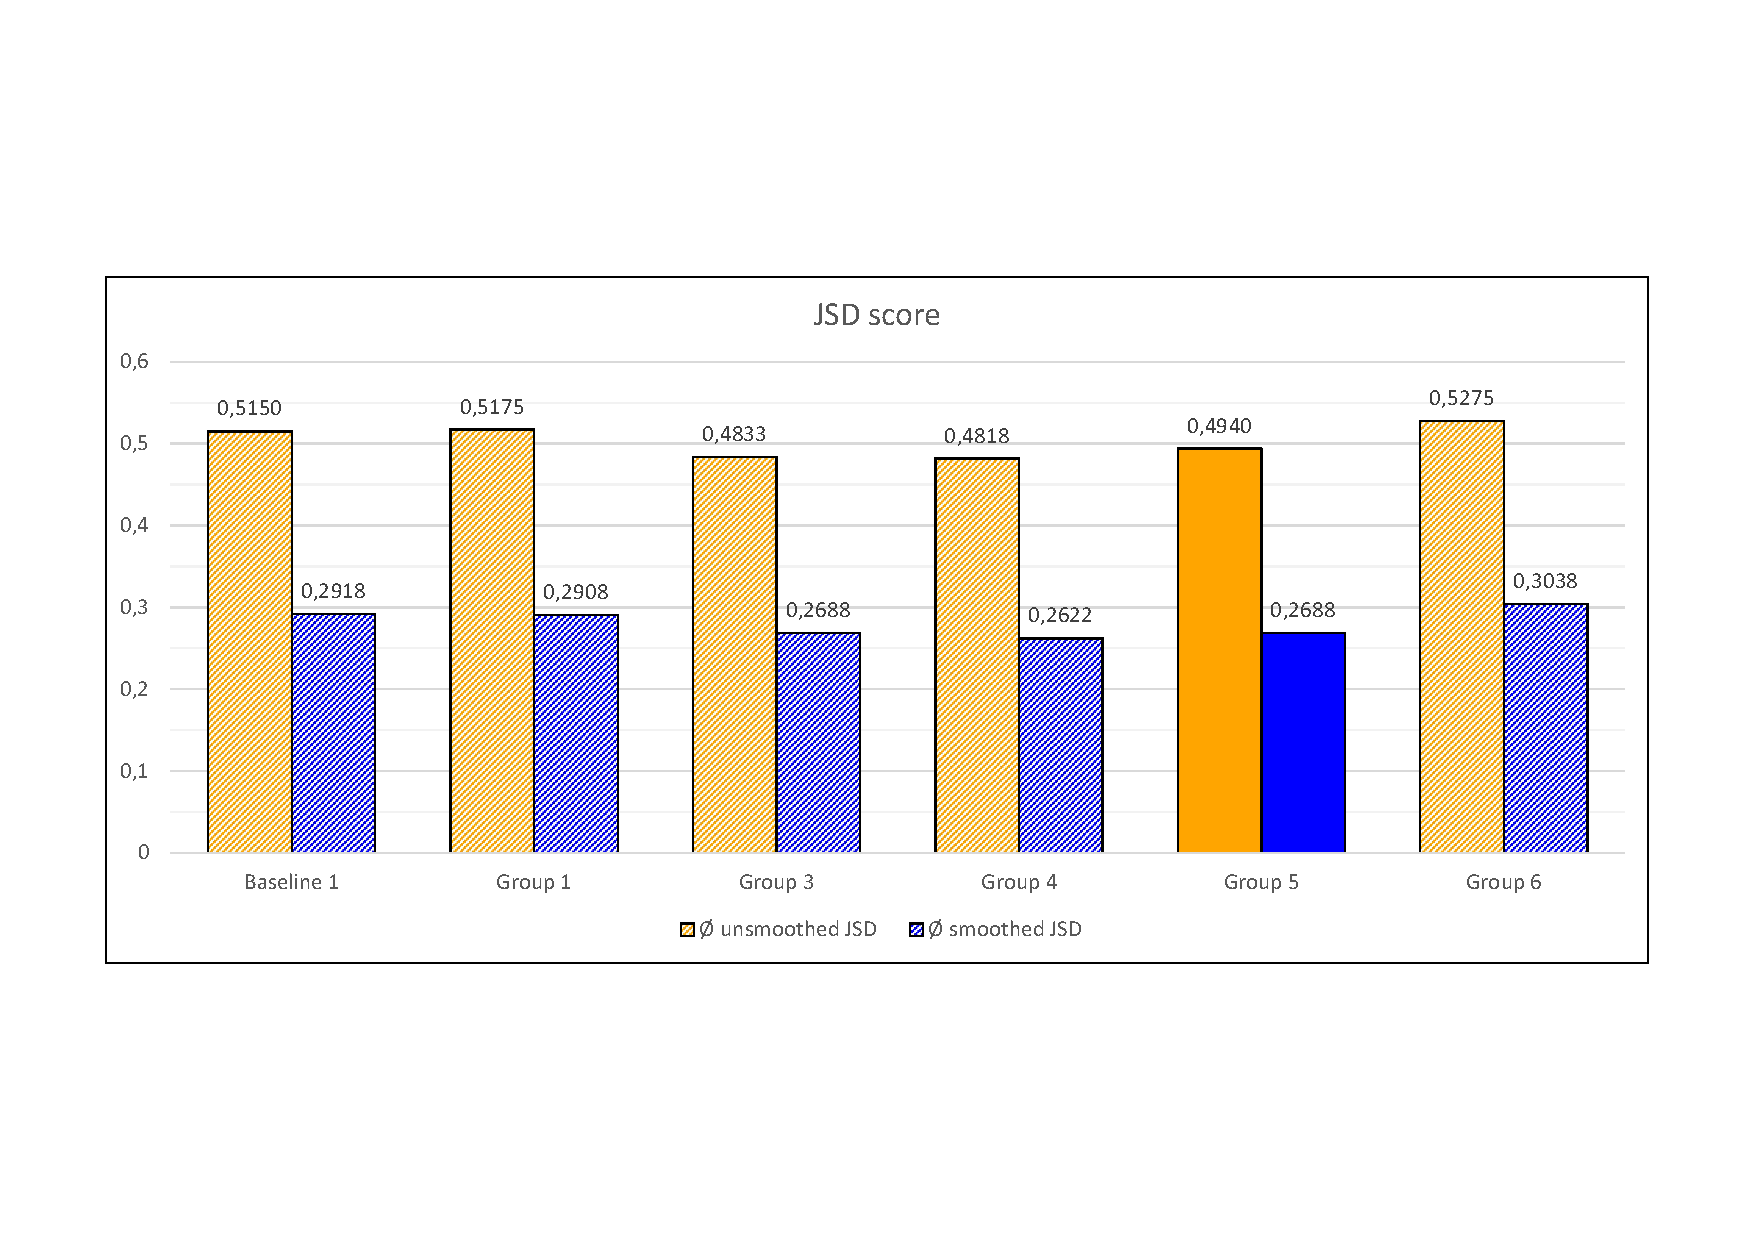
\includegraphics[trim=0 150 0 150, width=\textwidth]{img/jsd.pdf}
	\caption{JSD score}
	\label{fig:jsd}
\end{figure}


\subsection{Scores per Criteria}

We analyzed our average score per criteria against the average score per criteria over all groups. The results are shown in figure~\ref{fig:spc}.

\begin{figure}[H]
	\centering
	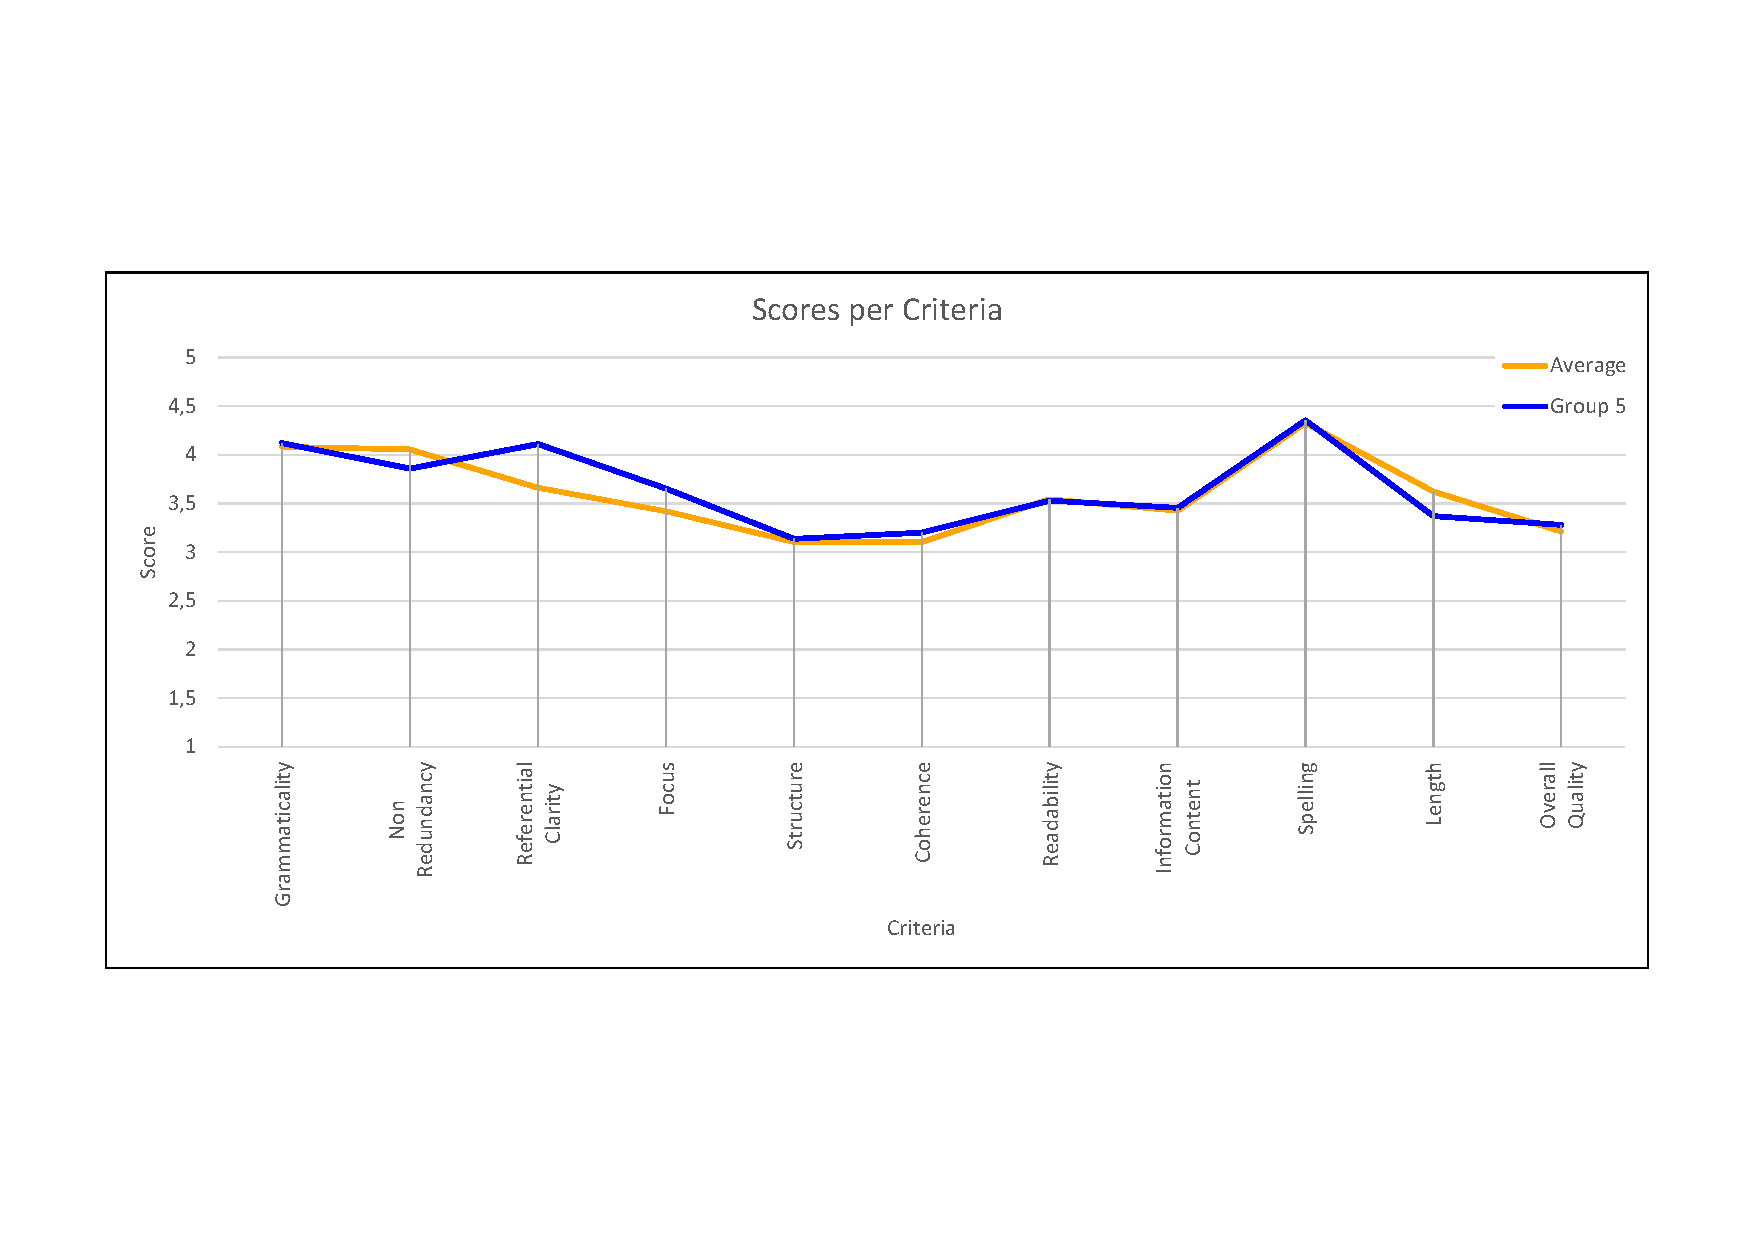
\includegraphics[trim=0 150 0 150, width=\textwidth]{img/scores_per_criteria.pdf}
	\caption{scores per criteria}
	\label{fig:spc}
\end{figure}

There are only two criteria our group is significant worse than the average, "non-redundancy" and "length". On the other hand there are several criteria we are better than the average, e.g. "referential clarity" or "focus".

For a better understanding of these values, we have to make a closer look at the free text comments.
In table~\ref{tab:evacomments} you can see an overview with all criteria, the number of comments for the criteria and the main points concerning the criteria. Furthermore, all comments are shown in appendix~\ref{appex:freetext}, grouped by criteria.

\begin{table}[H]
	\begin{tabularx}{\textwidth}{llX} \toprule
		criteria & \# & main point \\ \midrule
		Grammaticality      & 25 & punctuation incl. periods, parenthesis  \\
		Non-Redundancy      & 19 & repetition resp. multiple definitions \\
		Referential Clarity & 11 & unsolved reference \\
		Focus               & 17 & one sentence does not fit \\
		Structure           & 13 & order of sentences \\
		Coherence           & 9  & lack of information due to bad sentence connection \\
		Readability         & 21 & punctuation and too long sentences \\
		Information Content & 15 & one sentence does not fit \\
		Spelling            & 17 & punctuation and case-related problems \\
		Length              & 31 & not exactly 600 characters \\
		Overall Quality     & 14 & lack of information, structure, or length \\ \bottomrule
	\end{tabularx}
	\caption{evaluation criteria}
	\label{tab:evacomments}
\end{table}

It is noticeable, that there are some criteria that have a high number of comments and some with a low quantity.
This could be due to the complexity of the individual criteria, e.g "length" and "grammarticality" are easier to rate than "structure" or "coherence".

However, you can see that the annotators give more comments for criteria we are not so good at as for the other ones.
To evaluate the influence of the bad impressions, we have had a closer look to the "overall quality"-criteria.
Due to the construction of this criteria, the value should be nearly an average score of the other ten criteria.
So we calculated every average value of all criteria (except "overall quality") and compared it against the given "overall quality"-rating for each annotator.
The results are shown in figure~\ref{fig:deviation}.

\begin{figure}[H]
	\centering
	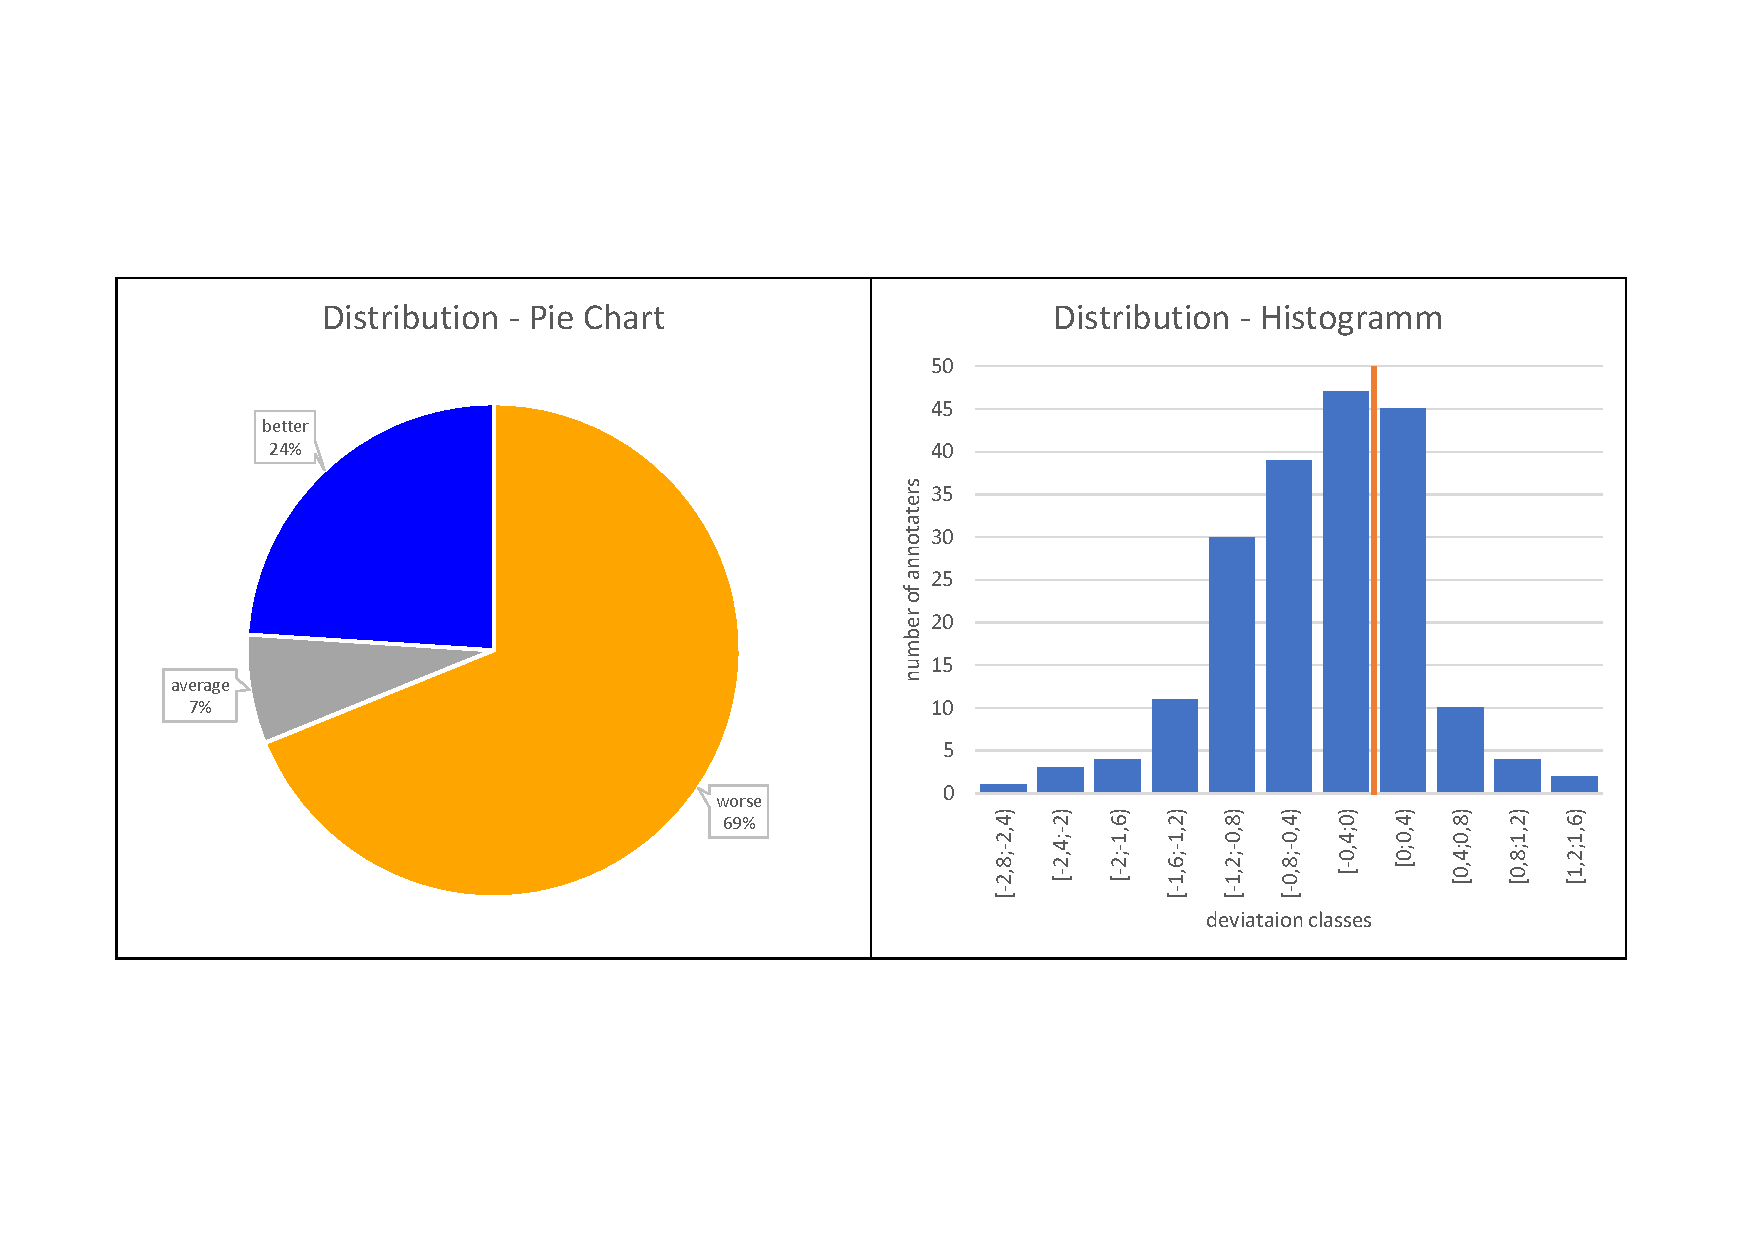
\includegraphics[trim=10 150 10 150, width=\textwidth]{img/deviation.pdf}
	\caption{scores per criteria}
	\label{fig:deviation}
\end{figure}

It is significant that more than two out of three annotators gave a worse score for "overall quality" than the average of the other criteria suggests.
To strengthen this impression, on the right hand side of figure~\ref{fig:deviation} you can see the distribution grouped by deviation classes. The vertical orange line indicates a deviation of zero. All classes have a range of 0.4.

It is noticeable that roughly half of the annotators (92 out of 196) rated near the average $\pm$ 0.4. But the deviation on the worse rated side is twice as much as on the better rated side.
The assumption that worse rated criteria influence the overall impression more than better rated ones has not been proven, but is very much strengthened.

Another special feature is noticeable when viewing the main points of the free comments.
The criteria are not independent of each other.
Punctuation is often written as bad influence for a criteria. Of course, punctuation is important for a good "grammaticality" result, but this criteria influences "readability" and "spelling", too.
On the other hand, "readability" is also influenced by "structure", "coherence", "spelling" and "grammaticality".
For an exhaustive evaluation of the dependencies of these criteria, there is too little information given, so this will have to examined in another study.


\subsection{Scores including the Weight and Confidence}
\label{eva:box}
To include the weight and confidence of the annotators for the single criteria we developed a formula to calculate an evaluation score per annotator for a summary.
$$score_{eval} = \frac{\sum_i score_i \times weight_i \times confidence_i}{\sum_i weight_i \times confidence_i}$$
Due to the construction of this formula the result is always a value between 1 and 5.

We calculate an evaluation score for all group and the baseline for every summary.
Further to see the statistical distribution we calculated the minimal and maximal score and the quantile $Q_{0.25}$, $Q_{0.50}$ and $Q_{0.75}$, also known as q1, q2 and q3.
The results are shown in table~\ref{tab:evascore}.
\begin{table}[H]
	\begin{tabularx}{\textwidth}{X|XXXXX} \toprule
		         & \multicolumn{5}{c}{quartile}                         \\
		group    & min      & q1       & q2       & q3       & max      \\ \midrule
		baseline & 1.550589 & 2.311526 & 2.603768 & 2.809197 & 3.211129 \\
		group 1  & 2.248760 & 2.690341 & 3.127374 & 3.470968 & 4.441776 \\
		group 3  & 2.608760 & 3.507732 & 3.752306 & 3.953384 & 4.576654 \\
		group 4  & 2.469870 & 3.233777 & 3.619146 & 4.000742 & 4.525670 \\
		group 5  & 2.037820 & 3.362673 & 3.713002 & 3.883326 & 4.470253 \\
		group 6  & 2.665251 & 3.288665 & 3.579060 & 3.834127 & 4.371757 \\ \bottomrule
	\end{tabularx}
	\caption{statistical distribution of the calculated evaluation score}
	\label{tab:evascore}
\end{table}

As written in \citet{vis_mem} a box plot is a very good visualization for a statistical distribution.
According to this fact, we converted the data listed in table~\ref{tab:evascore} into a box plot to show the distribution and to have a good opportunity to compare the quality of each group against the other groups. The resulting visualization is shown in figure~\ref{fig:box}.

\begin{figure}[H]
	\centering
	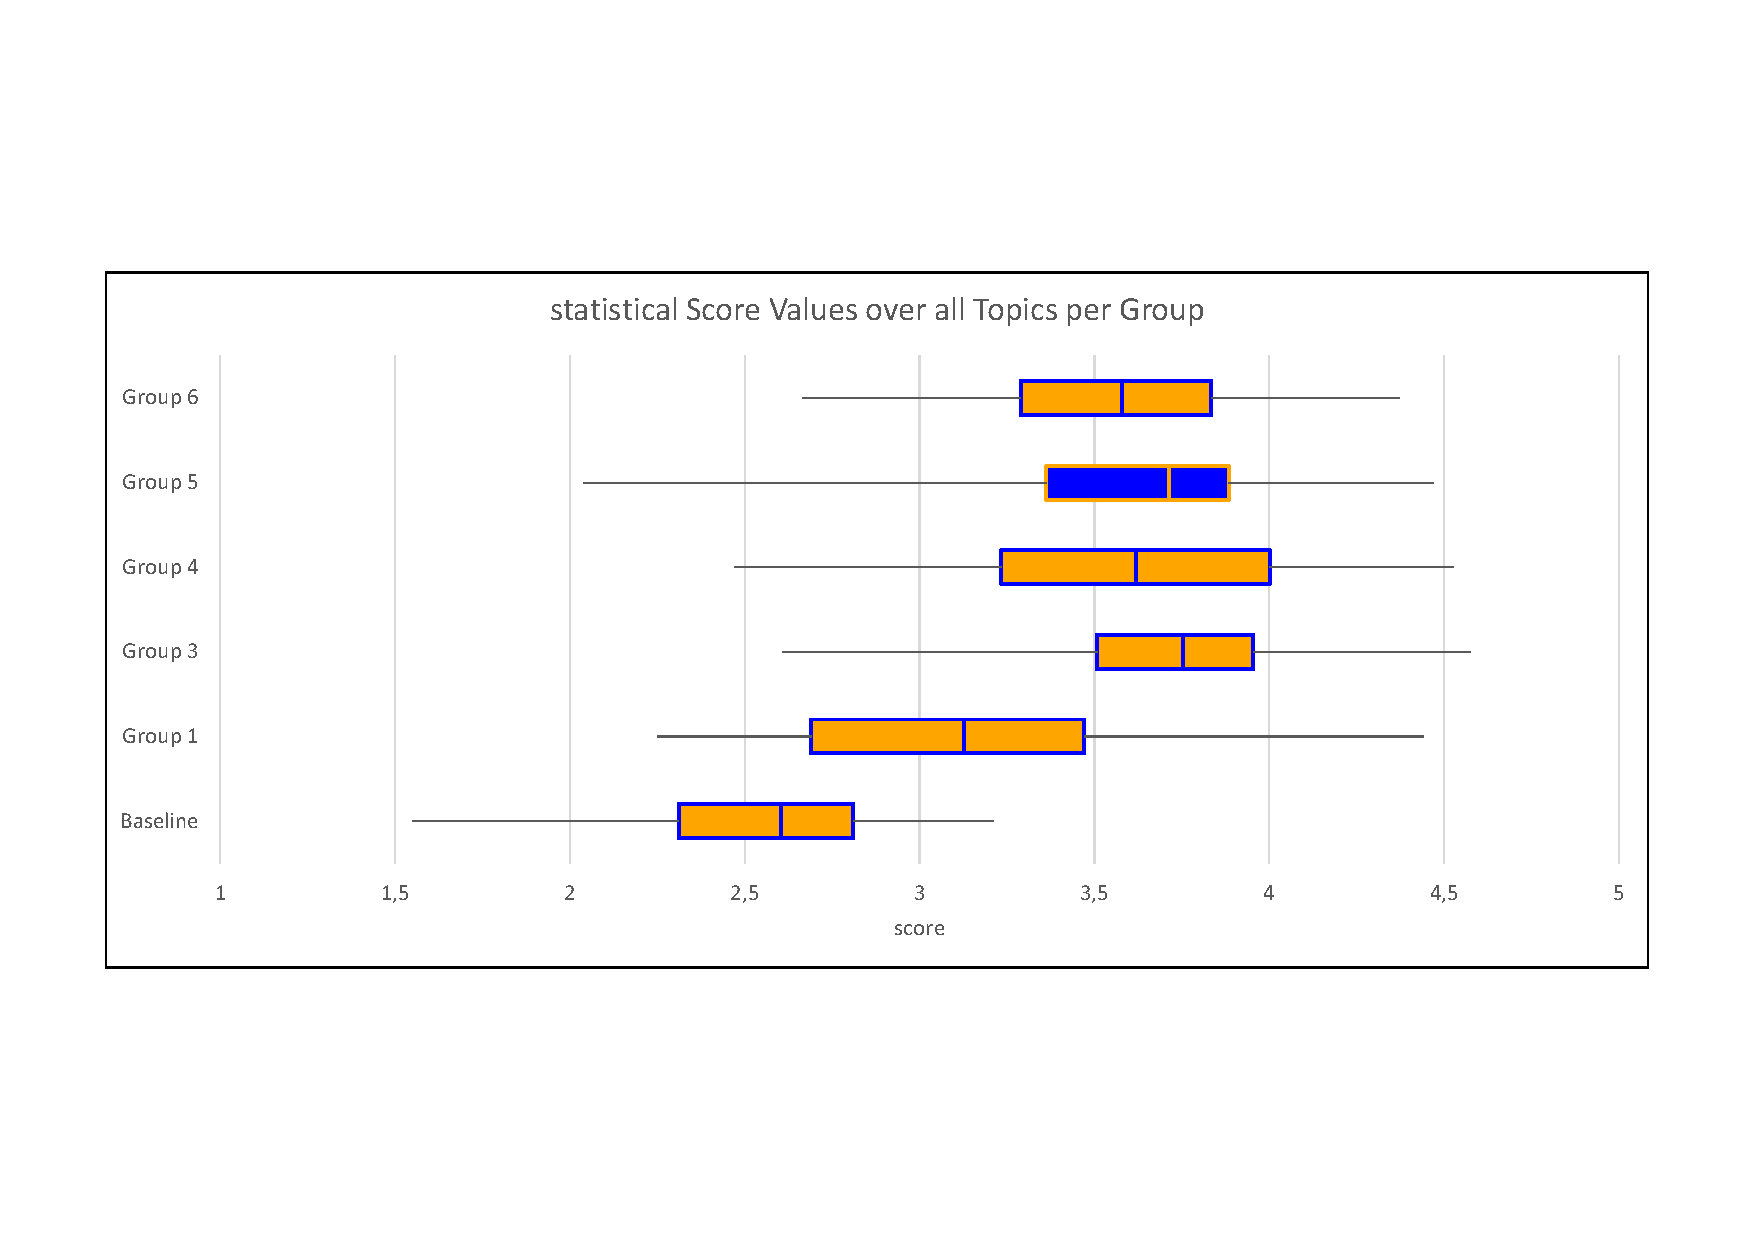
\includegraphics[trim=0 150 0 150, width=\textwidth]{img/box.pdf}
	\caption{statistical values over all topics per group}
	\label{fig:box}
\end{figure}

As you can see in figure~\ref{fig:box} the median for our group has almost the highest value. Due to the construction of the median, it shows "middle" value for a data set. Therefore our summaries are quite good compared to the others.
The interquartile range for our group is also good with a value of 0.5, so 50\% of our summaries are near the "middle" value with an acceptable deviation.
The whiskers have to be considered individually.
On the one hand, the whisker indicating the range of q3 to the maximum value is similar to the same whiskers of the other groups, i.e., each group has some very good summaries, but the they are not significant.
On the other hand the whisker indicating the range of the minimum value to the q1 is enormous.
That means there some bad summaries, but they are so bad, they cannot be compared to the majority of the results.

A closer look to our box shows that the data for our group is left-skewed.
That means that the data is not normally distributed, but the majority of the data has a higher score value.

For all groups you can see, that they are better as the baseline and most of the summaries have a rating between 3.5 and 4.0.

\subsection{Score Calculation for each Topic}

As shown in the section before our group achieved a very good result with most of our summaries.
To determine the best summary and the worst summary we calculated the score per topic with the formula shown in section~\ref{eva:box}. The results are visualized in figure~\ref{fig:spt}.

\begin{figure}[H]
	\centering
	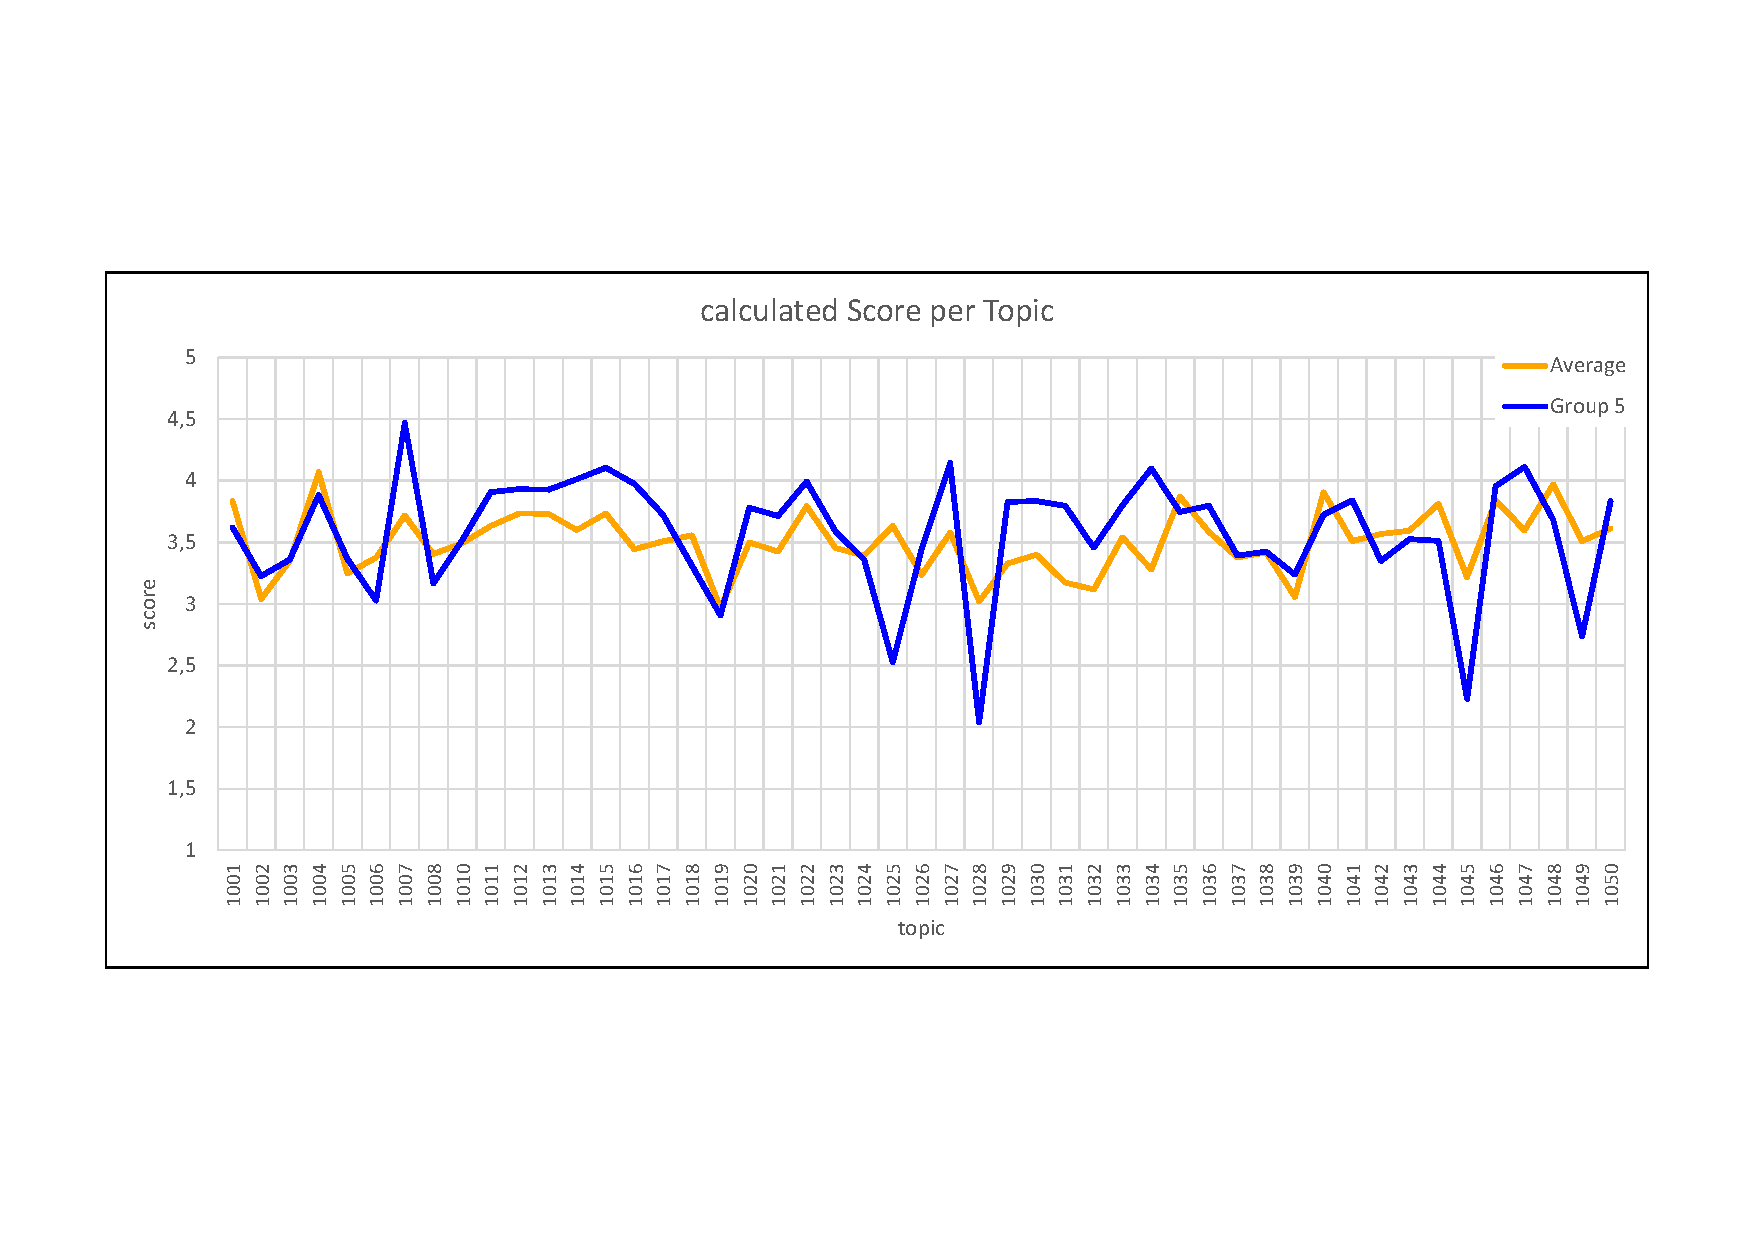
\includegraphics[trim=0 150 0 150, width=\textwidth]{img/score_per_topic.pdf}
	\caption{scores per topic}
	\label{fig:spt}
\end{figure}

In figure~\ref{fig:spt} you can see, that our calculated score is near the average score of all groups, but often higher. This reflects the left-skewed distribution you can see in the box plot (figure~\ref{fig:box}).
The length of the whiskers can be also explained with the results of this calculation.
Topic 1007 limits the right whisker with a top value of approx. 4.5.
The length of the left whisker can be explained with the value of topic 1028 (approx 2.0).

Furthermore, we sorted the data for our group and the average value data, independent from each other, to affirm the special feature, that the data is left-skewed. The corresponding visualization is shown in figure~\ref{fig:spts}.

\begin{figure}[H]
	\centering
	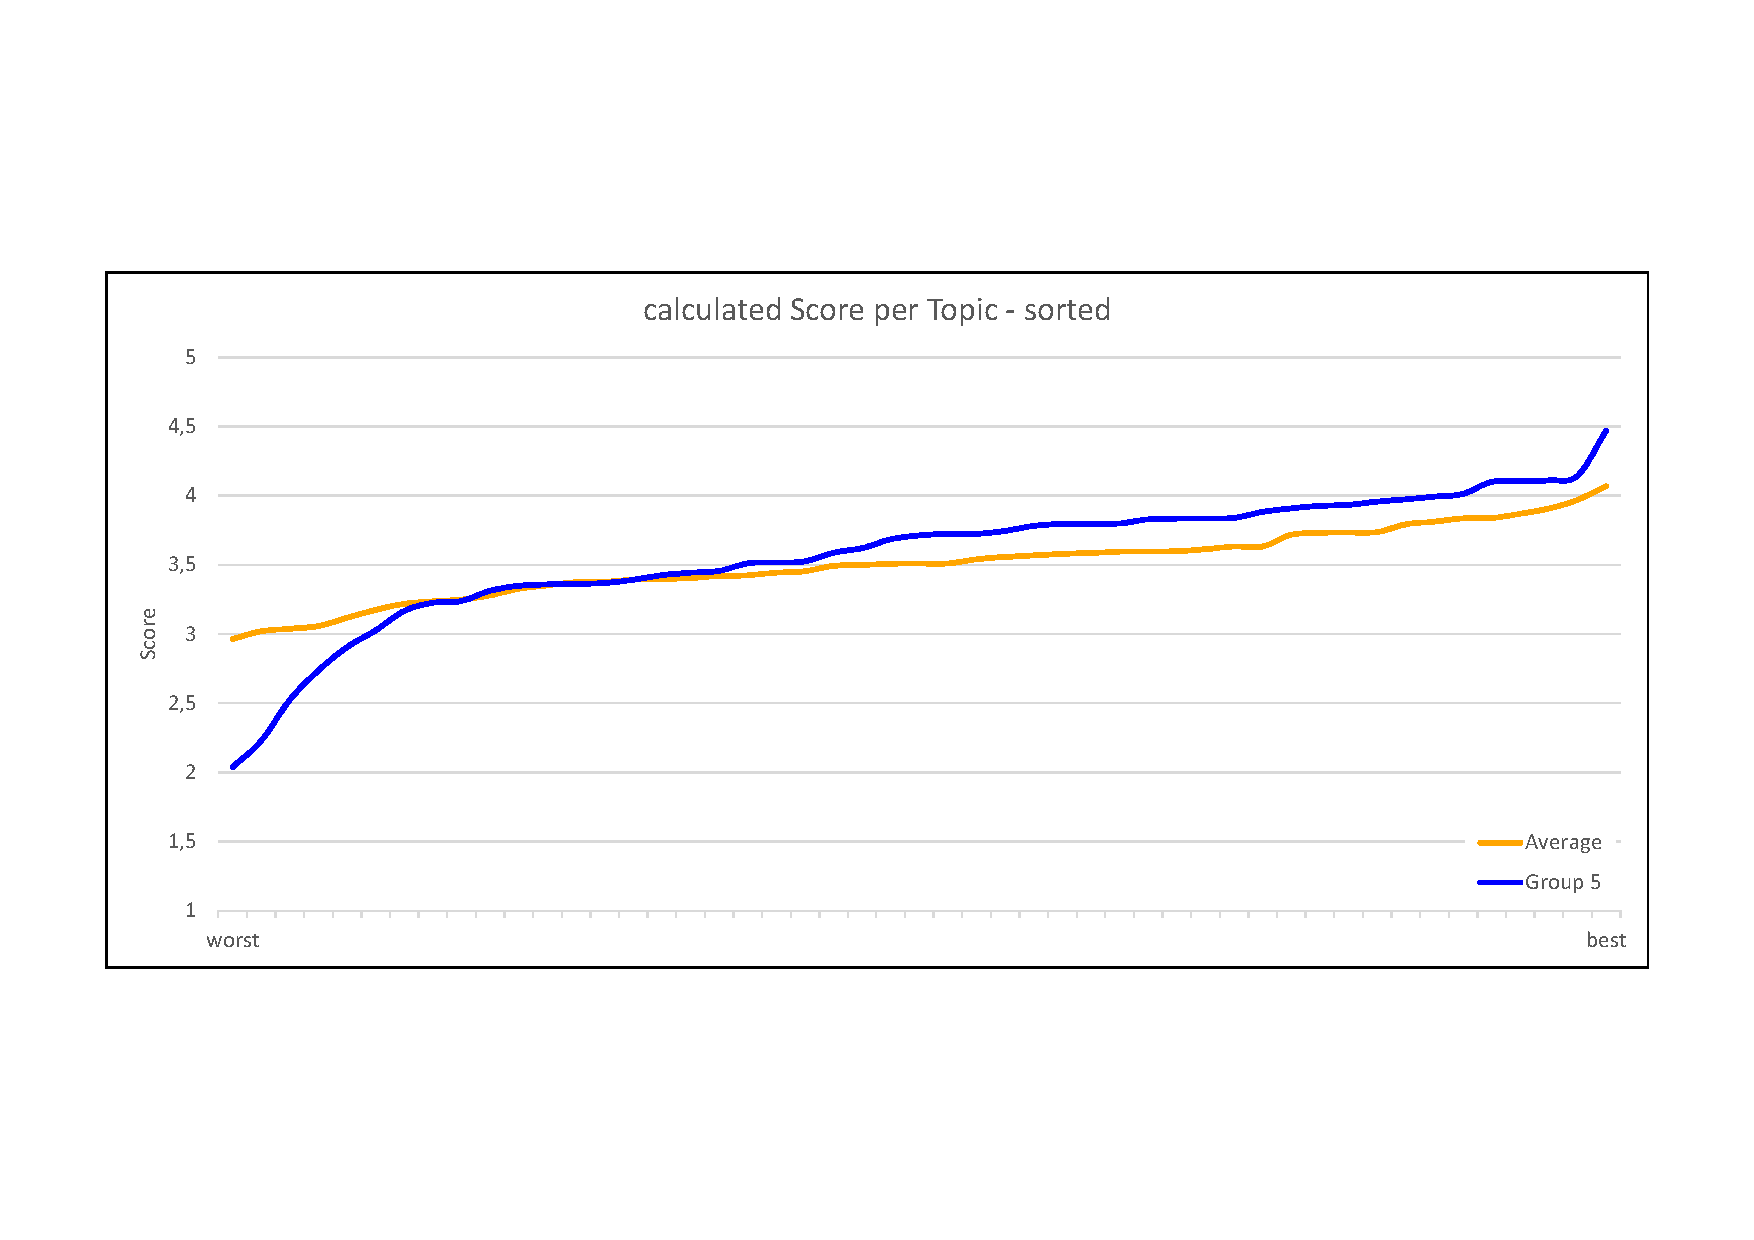
\includegraphics[trim=0 150 0 150, width=\textwidth]{img/score_per_topic_sorted.pdf}
	\caption{scores per topic sorted ascending}
	\label{fig:spts}
\end{figure}

In figure~\ref{fig:spts} you can also see the influence of the worst and best rated topic on the length of the whiskers.
As a further result, you can see that only twelve summaries are worse than the average and 26 summaries are better than the average with a margin of at least 0.175.

\subsection{Worst and Best Summary}
To complete the evaluation we print our worst and best summary below.

\subsubsection*{our \emph{worst} summary - topic 1028: "parents' involvement in children alcohol behavior"}
\fbox{\begin{minipage}{\textwidth}
	The parents are exhibiting some serious problems as well, such as drug abuse,
	alcohol abuse, criminal involvement, and domestic violence. \\
	teen discipline, teen boot camp, alcohol abuse, Binge Drinking, Substance Abuse,
	Addiction, bad behavior, boot camp, children respect, parenting tips, aggressive
	behavior, James Lehman, Total Transformation Individuals suffering from mental
	health disorders may use alcohol and illicit drugs to decrease or mitigate their
	psychological distress 16 .
\end{minipage}}

Our summary of topic 1028 is rated with a score of 2.037819, the average score is 3.019711.

\vspace{1em}
\subsubsection*{our \emph{best} summary - topic 1007: "getting rid of childhood phobia"}
\fbox{\begin{minipage}{\textwidth}
		Fears and Phobias can be resolved with hypnosis and hypnotherapy Hypnotherapy
		is an ideal option because it is safe, effective, and non-invasive. \\
		If a parent is afraid of spiders then a child can learn that fear and it could develop
		into a phobia. \\
		Hypnotherapy is effective at helping you to overcome your fear by treating the
		anxiety caused by the trigger, and by re-training the mind to remember the original
		trigger in a way that does not create anxiety. \\
		Medication can be very effective in treating phobias, especially social phobia and
		agoraphobia.
\end{minipage}}

Our summary of topic 1007 is rated with a score of 4.470253, the average score is 3.718157.

\subsection{Conclusion}

We analyzed our results in multiple ways to stress out several shortcomings and advantages of our approach to this task. Our evaluation shows that we had a better quality score than the baseline. The median of the overall quality of our rated summaries was 3.7 and this indicates that our system produces good result.